\chapter{Erweiterte Untersuchungen}

\section{Einfluss der Anzahl der Fingerprints}
\begin{itemize}
    \item \textbf{Untersuchungsszenario:} Beschreiben Sie das Szenario zur Untersuchung des Einflusses der Fingerprint-Anzahl.
    \item \textbf{Datenerhebung:} Erklären Sie, wie die zusätzlichen Fingerprints gesammelt wurden.
    \item \textbf{Analyse und Ergebnisse:} Diskutieren Sie die Analyse und die Ergebnisse der Untersuchung.
\end{itemize}

\section{Analyse von nahe beieinanderliegenden Räumen}
\begin{itemize}
    \item \textbf{Untersuchungsszenario:} Beschreiben Sie das Szenario zur Untersuchung der Genauigkeit bei nahe beieinanderliegenden Räumen.
    \item \textbf{Datenerhebung:} Erklären Sie, wie die Daten für diese Untersuchung gesammelt wurden.
    \item \textbf{Analyse und Ergebnisse:} Diskutieren Sie die Analyse und die Ergebnisse der Untersuchung.
\end{itemize}

\section{Einfluss von Flur-Messungen auf False Positives}
\begin{itemize}
    \item \textbf{Untersuchungsszenario:} Beschreiben Sie das Szenario zur Untersuchung des Einflusses von Flur-Messungen.
    \item \textbf{Datenerhebung:} Erklären Sie, wie die Flur-Messungen durchgeführt wurden.
    \item \textbf{Analyse und Ergebnisse:} Diskutieren Sie die Analyse und die Ergebnisse der Untersuchung.
\end{itemize}

\subsection{Flur/Nicht Wahr etc.}

Die Ergebnisse der verschiedenen Strategien zur Auswahl des Flur/Nicht Wahr etc. sind in Abbildung \ref{fig:8_test_corrdior_01} dargestellt.

\begin{itemize}
    \item Bisher wurden nur Messungen in Räumen vorgenommen und es wurde überprüft, ob der Raum korrekt vorhergesagt wurde
    \item weiterer Ansatz: Die API kann auch vorhersagen, dass nichts vorhergesagt werden kann, sodass klar ist, dass die Vorhersage nicht falsch ist
    \item Dafür wird neben True/False auch Not False eingeführt
\end{itemize}    

\begin{figure}[H]
    \centering
    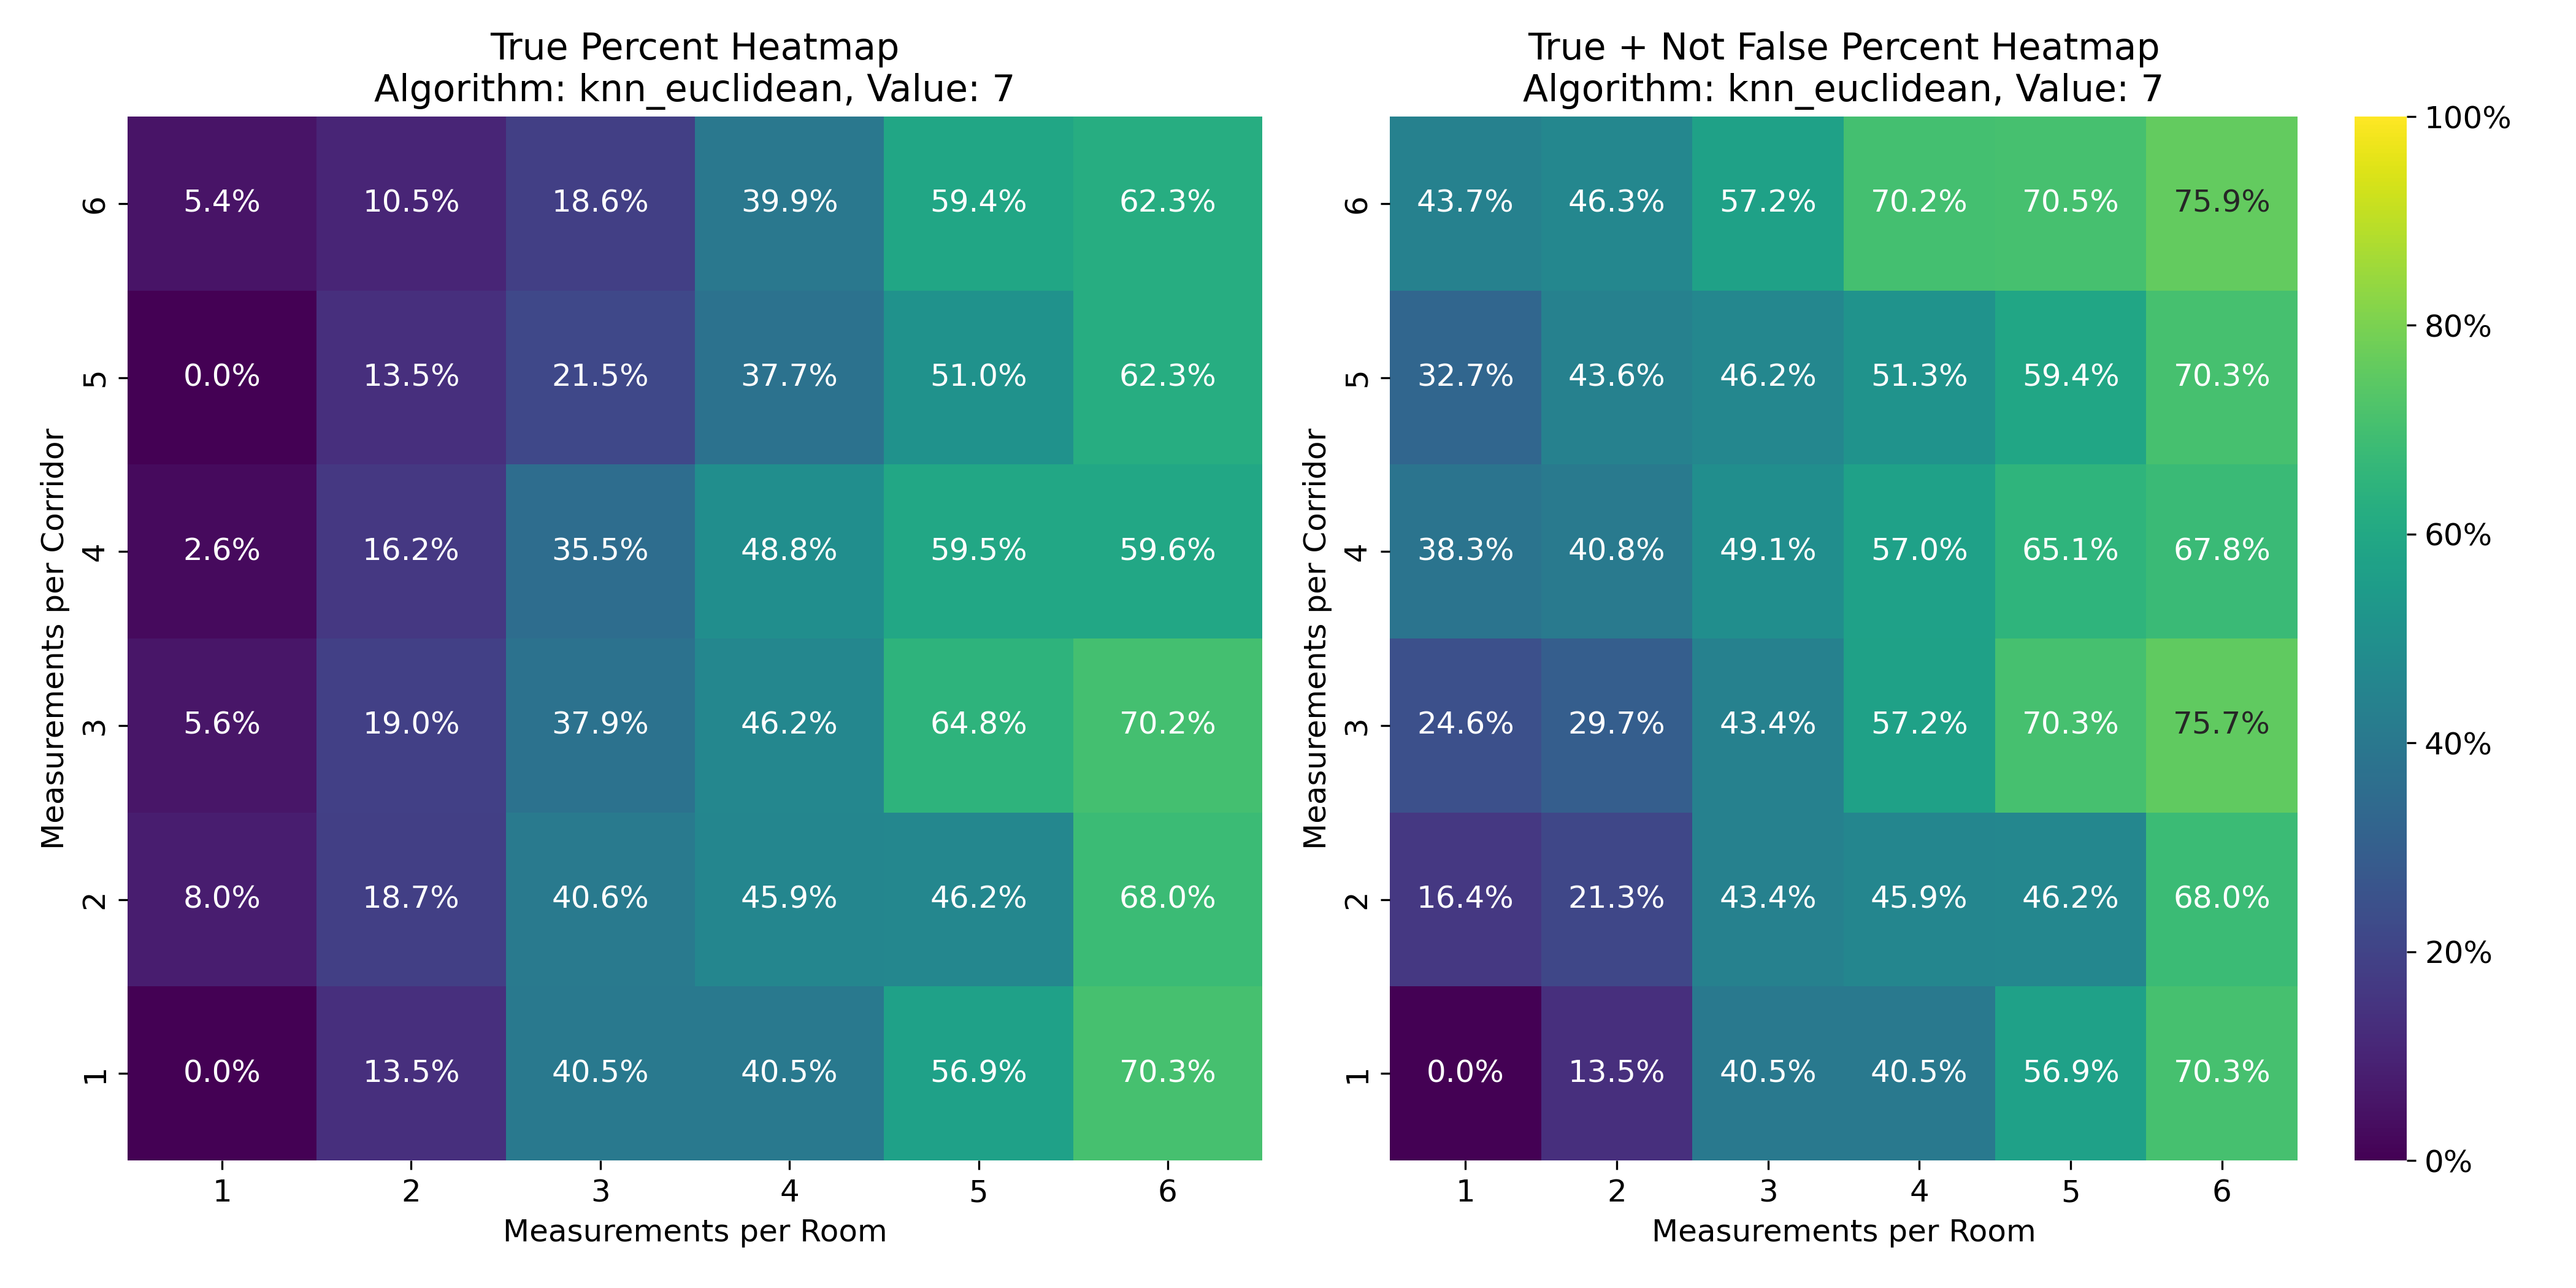
\includegraphics[width=0.8\textwidth]{images/8_test_corrdior_01.png}
    \caption{Flur/Nicht Wahr etc.}
    \label{fig:8_test_corrdior_01}
\end{figure}

\section{Optimale Algorithmen und Einstellungen}
\begin{itemize}
    \item \textbf{Zusammenfassung der besten Algorithmen:} Fassen Sie die Ergebnisse der vorherigen Untersuchungen zusammen.
    \item \textbf{Empfohlene Einstellungen:} Erklären Sie die empfohlenen Algorithmen und Einstellungen basierend auf den Ergebnissen.
    \item \textbf{Schlussfolgerungen:} Diskutieren Sie die Schlussfolgerungen und Implikationen für die Anwendung der Algorithmen.
\end{itemize}
